\documentclass{acm_proc_article-sp}

\usepackage{graphicx}
\graphicspath{ {images/} }

\begin{document}

\title{Subway Spot Selection}
\subtitle{A Behavioral Model}

\numberofauthors{1} 
\author{
\alignauthor
       Dan Gopstein\\
       \affaddr{New York University}\\
       \email{dgopstein@nyu.edu}
}

\date{December 2014}


\maketitle
\begin{abstract}
We introduce a behavioral model of the subway passenger that describes their spot selection process upon on boarding the train car. We propose that passengers choose their spot based on a mixture of environmental and social factors. We go on to analyze the social optimization problem as a resource selection game.
\end{abstract}

\section{Introduction}
The New York City Subway system provides, on average, over 5 million rides every weekday~\cite{MTAFacts}. The interior design of subway cars has a daily impact on millions of urban commuters. Subway car utilization is an important factor in public transit ecosystem of many large cities. Previous work has focused on observational studies of topics from spot selection\cite{berkovich2013observed} to physiological reactions\cite{evans2007crowding} to race\cite{maines1979ecological} and sex\cite{hai1982sex} issues. Relatively less researched have been the underlying models that humans use to make these decisions. Through observational data (kindly provided by Alex Lu of Berkovich, Lu, Levine, Reddy), user studies and intuition garnered from psychological research\cite{evans2007crowding, hai1982sex, maines1979ecological} we have created and validated a computational model of the subway passengers decision making process. Using this model we then translate the human value system into an objective function that we use in an economic model based off techniques in resource selection.

[Describe the "Spot Selection Game"]

\section{Behavioral Model}
Before developing an accurate economic model of the Spot Selection Game, we first had to understand the factors that motivate the passengers themselves. There were two major data sets used in generating our model. First, were the observed passenger data from Berkovich, et al. Second were responses from a survey that we designed to help understand which design factors were important when passengers made their spot selection.

\subsection{Observed Passenger Data}
The most significant data set used to build the decision model was that provided by Berkovich, et al. Their team rode subway cars and manually annotated forms describing the positions of each sitting and standing passenger on subway cars for individual stops along several routes. For a more thorough description of their methods, see their report\cite{berkovich2013observed}. In total they recorded 1925 passenger positions for 62 stops, over 45 stations, on 15 lines, in 11 classes of car. In our usage of of Berkovich, et al's data, there are some situations such as inferring patterns where we used the entire data set, and other situations, such as verifying the results of our simulations, where we only used data from the single most heavily observed car class, the R68, for which 14 stops' passengers were observed.

\subsection{Decision Motivation Survey}
In order to inform the design of our passenger decision model, we solicited descriptions of 15 subway passenger's own thoughts on where they choose to sit or stand, and why they made those decisions. The survey was broken up into two sections. First, the participants were asked rank, in order of preference, which seats or standing positions they preferred on a given subway car. Then, they were asked to describe which factors most influenced their decision to sit or stand, and about their relative preference stand versus sit when possible.

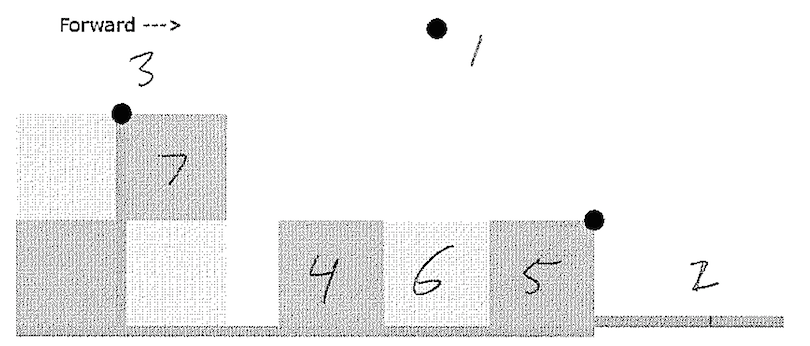
\includegraphics{survey_response}

\section{Results and Discussions}
Through user studies, surveys and predictive modeling we developed an object that mimics the behavior of passengers on the R68 subway car.

\bibliographystyle{abbrv}
\bibliography{subway}

%\balancecolumns 

\end{document}
